\section{Fondamenta degli Algoritmi Quantistici}
In questa sezione viene descritto quali sono e come vengono eseguite
le computazioni su un computer quantistico. Inizialmente vengono analizzate
le differenze che si hanno quando ci si confronta con un modello di computazione classico
e, nello specifico, verranno elencati algoritmi quantistici che offrono
vantaggi rispetto ad una computazione classica.
\subsection{Computazione classica vs Computazione quantistica}
Uno dei primi vantaggi che una computazione quantistica può offrire
è sicuramente quello del \textbf{tempo}; infatti, per alcuni problemi, sono state proposte
nuove soluzione che hanno dimostrato un incremento esponenziale del tempo di esecuzione.

Mediante l'utilizzo di porta logica di \textbf{Toffoli}, è possibile simulare circuiti 
logici classici su circuiti quantistici. La porta di \textbf{Toffoli} riesce
ad implementare un qualsiasi circuto Booleano; inoltre, la reversibilità di tale porta,
contribuisce alla simulazione dei circuiti classici su circuiti quantistici.

Ad esempio, riusciamo a simulare la porta NAND (irreversibile) con la porta di Toffoli.
La figura \ref{fig13} mostra il NAND implementato con il Toffoli gate.
\begin{figure}[h]
    \centering
    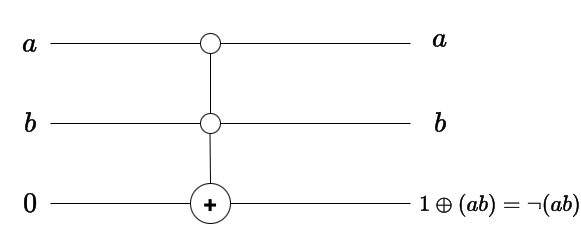
\includegraphics[width = 7cm]{./Images/toff.png}
    \caption{}
    \label{fig13}
\end{figure}

\begin{fact}{}{}
    È possibile implementare qualsiasi circuito booleano classico attraverso la porta di Toffoli.
\end{fact}

\subsection{Parallelismo Quantistico}
Data una funzione $f(x)$, definiamo (a parole semplici) il \textbf{parallelismo
quantistico} come una caratteristica del mondo quantistico che permette
la valutazione di $f(x)$ per diversi valori di $x$ simultaneamente.

Supponiamo che $f(x): \{0,1\} \rightarrow \{0,1\}$. Calcolare tale funzione
in un'ambiente quantistico necessita la definizione di un'operazione 
unitaria, solitamente chiamata $U_f$, rappresentata nella figura \ref{fig14}.
\begin{figure}[h]
    \centering
    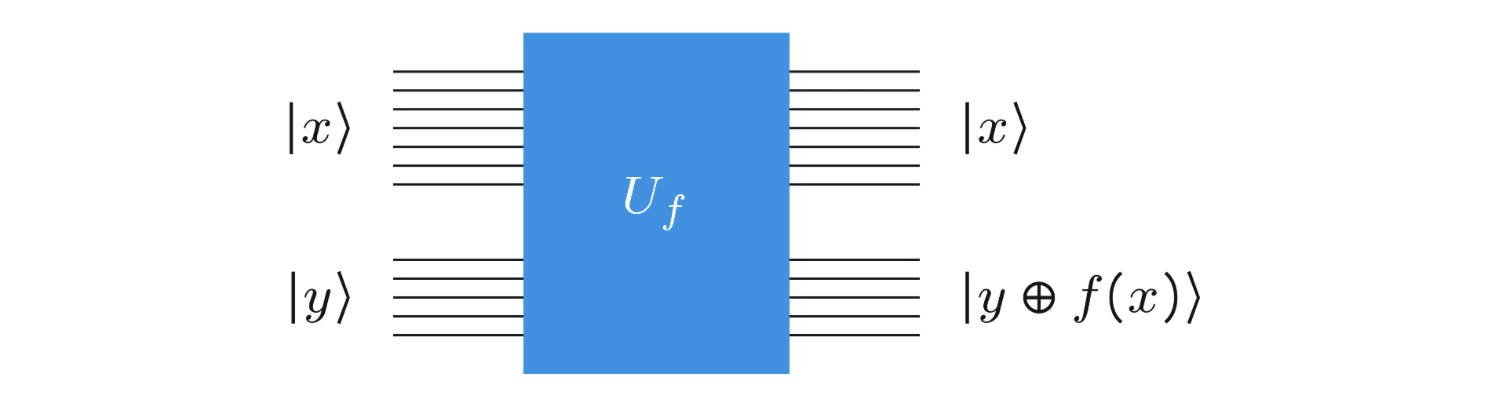
\includegraphics[width = 10cm]{./Images/uf.png}
    \caption{}
    \label{fig14}
\end{figure}
 Quindi dobbiamo considerare un computer quantistico a due qubit,
 che inizializza lo stato a $|x,y\rangle$. 
 
 Dopo l'applicazione di $U_f$, riusciamo a trasformare lo stato in $|x,y \oplus f(x)\rangle$, 
 dove $\oplus$ indica l'operazione \textit{bitwise} dello XOR. Denominiamo il primo registro come
 \textit{data} e il secondo come \textit{target}.

 \begin{oss}{}{}
    Se $y=0$, allora lo stato finale del secondo qubit è equivalente
    ad $f(x)$.
 \end{oss}

 Supponiamo ora che inizializziamo il registro \textit{data} nella superposizione
 \begin{equation*}
    |+\rangle = \frac{1}{\sqrt{2}}|0\rangle + \frac{1}{\sqrt{2}}|1\rangle
 \end{equation*}
 la quale può essere ottenuta, ad esempio, applicando la porta di Hadamard
 sullo stato base $|0\rangle$. Supponiamo anche di inizializzare il ragistro
 \textit{target} con $|0\rangle$. Quindi:
 \begin{equation*}
    \begin{array}{c}
        U_f\left(\left(\frac{1}{\sqrt{2}}|0\rangle + \frac{1}{\sqrt{2}}|1\rangle\right)\otimes |0\rangle\right) = \frac{1}{\sqrt{2}}\left(U_f \left(|0\rangle \otimes |0\rangle\right) + U_f \left(|1\rangle \otimes |0\rangle\right)\right) \\ \\
        = \frac{1}{\sqrt{2}}\left(|0\rangle \otimes |f(0)\rangle + (|1\rangle \otimes |f(1)\rangle)\right)
    \end{array}
 \end{equation*}
 Osserviamo, incredibilmente, di come ci sia bastata una singola 
 valutazione per computare la funzione su tutto il dominio della funzione ($\{0,1\}$).
 Abbiamo semplicemente sfruttato l'abilità di un qubit di stare
 in una superposizione tra stati differenti.

 Questa procedura è generalizzabile per tutte le funzioni aventi
 un numero arbitrario di bits, utilizzando un'operazione
 generale conosciuta come \textbf{trasformazione di Hadamard}, o anche
 \textbf{trasformazione di Walsh-Hadamard}. È semplicemente l'applicazione 
 di $n$ porte di Hadamard in parallelo su $n$ qubits.
 \begin{example}{}{}
    Ad esempio, per $2$ qubit inizializzati allo stato base $|0\rangle$,
    la trasformazione ci da come output:
    \begin{equation*}
        \left(\frac{|0\rangle + |1\rangle}{\sqrt{2}}\right)\left(\frac{|0\rangle + |1\rangle}{2}\right) = \frac{|00\rangle + |01\rangle +|10\rangle +|11\rangle}{\sqrt{2}}
    \end{equation*}
 \end{example}
 Nel esempio, denotiamo con $H^{\otimes 2}$ l'operazione parallela delle porte di Hadamard. Più in generale, 
 la computazione di tale trasformazione su $n$ qubit con stato di partenza a $|0\rangle$ è equivalente a
 \begin{equation*}
    \frac{1}{\sqrt{2^n}}\sum_{x \in \Sigma} |x\rangle
 \end{equation*}
ed indichiamo con $H^{\otimes n}$ tale operazione. Otteniamo una superposizione di
\textbf{$2^n$} stati usando solo \textbf{$n$} porte.

La misurazione dello stato $\frac{1}{\sqrt{2^n}}\sum_{x \in \Sigma} |x\rangle$ ci restituisce solo $f(x)$, per un singolo
valore $x$. Non ci è tanto utile, quindi è necessaria l'abilità di estrazione di informazioni
su più di un valore di $f(x)$ dalla superposizione per poter sfruttare questo parallelismo.

\subsection{Algoritmo di Deutsch}
L'algoritmo di Deutsch, proposto da David Deutsch, è il primo algoritmo quantistico che dimostra 
quanto i circuiti quantistici performino meglio dei circuiti classici.

Sia $f: \{0,1\} \rightarrow \{0,1\}$. Come abbiamo visto in precedenza, esistono 4 tipi di funzioni di questo tipo:
\begin{equation*}
    \begin{array}{c|c}
        a & f_1(a) \\
        \hline
        0 & 0 \\
        0 & 0
    \end{array}
    \quad
    \begin{array}{c|c}
        a & f_2(a) \\
        \hline
        0 & 0 \\
        0 & 1
    \end{array}
    \quad
    \begin{array}{c|c}
        a & f_3(a) \\
        \hline
        0 & 1 \\
        0 & 0
    \end{array}
    \quad
    \begin{array}{c|c}
        a & f_4(a) \\
        \hline
        0 & 1 \\
        0 & 1
    \end{array}
\end{equation*}
che rappresentano rispettivamente la costante 0, la funzione identità, la funzione di negazione e la costante 1.
Definiamo la prima e l'ultima funzione come \textbf{costanti}, e la seconda e terza funzione come \textbf{bilanciate}.

\begin{definition}{Problema di Deutsch}{}
    Data in input una funzione $f: \{0,1\} \rightarrow \{0,1\}$, definiamo come \textbf{problema di Deutsch} il
    determinare se tale funzione è \textbf{costante} o \textbf{bilanciata}. 
\end{definition}
L'output di tale algoritmo ci darà $0$ se $f$ è costante, $1$ se $f$ è bilanciata. Associamo, per ogni funzione, la stringa
$f(0)f(1)$:
\begin{equation*}
    \begin{array}{c|c}
        \textbf{funzione} & \textbf{stringa} \\
        \hline
        f_1 & 00 \\
        f_2 & 01 \\
        f_3 & 10 \\
        f_4 & 11 
    \end{array}
\end{equation*}
Osserviamo che tale associazione funzione-stringa formi uno \textbf{XOR} nel nostro algoritmo.

Un qualsiasi algoritmo classico, richiede la valutazione di $f$ almeno per 2 volte, una per $f(0)$ e l'altra per 
$f(1)$. Nel mondo quantistico, riusciamo ad ottenere il risultato corretto con una sola valutazione di $f$.

\subsubsection{Implementazione}
\begin{figure}[h]
    \centering
    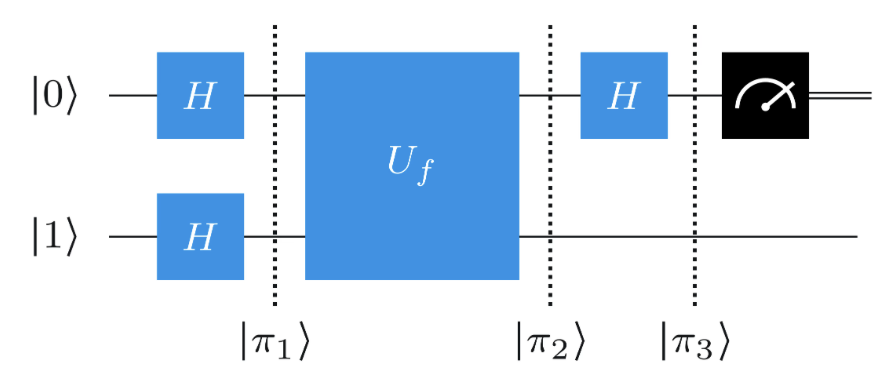
\includegraphics[width = 10cm]{./Images/deutch.png}
    \caption{}
    \label{fig15}
\end{figure}

La Figura \ref{fig15} mostra l'implementazione del circuito dell'algoritmo. Come prima, utilizziamo
la porta di Hadamard per preparare il primo qubit nella superposizione $|+\rangle$; questa volta prepariamo
anche il secondo qubit nella superposizione $|-\rangle$. Quindi avremo che:
\begin{equation*}
    |\pi_1\rangle = |+\rangle|-\rangle =  \left[\frac{|0\rangle + |1\rangle}{\sqrt{2}}\right]\left[\frac{|0\rangle - |1\rangle}{\sqrt{2}}\right]
    = \frac{1}{2}\left(|0\rangle - |1\rangle\right)|0\rangle + \frac{1}{2}\left(|0\rangle - |1\rangle\right)|1\rangle
\end{equation*}
Il prossimo passo è l'esecuzione di $U_f$, che trasforma lo stato in
\begin{equation*}
    |\pi_2\rangle = \frac{1}{2}\left(|0 \oplus f(0)\rangle - |1 \oplus f(0)\rangle \right)|0\rangle + \frac{1}{2}\left(|0 \oplus f(1)\rangle - |1 \oplus f(1)\rangle \right)|1\rangle
\end{equation*}
Sapendo che:
\begin{equation*}
    |0 \oplus a\rangle - |1 \oplus a\rangle = (-1)^a(|0\rangle - |1\rangle)
\end{equation*}
quindi che:
\begin{equation*}
    \begin{array}{c}
        |0 \oplus 0\rangle - |1 \oplus 0\rangle = (-1)^0(|0\rangle - |1\rangle) \\ \\
        |0 \oplus 1\rangle - |1 \oplus 1\rangle = (-1)^1(|0\rangle - |1\rangle)

    \end{array}
\end{equation*}
allora possiamo scrivere lo stato $\pi_2\rangle$ come:
\begin{equation*}
    \begin{array}{l}
        |\pi_2\rangle = \frac{1}{2}(-1)^{f(0)}(|0\rangle - |1\rangle)|0\rangle + \frac{1}{2}(-1)^{f(1)}(|0\rangle - |1\rangle)|1\rangle \\ \\
        = |-\rangle \left(\frac{(-1)^{f(0)}|0\rangle + (-1)^{f(1)}|1\rangle}{\sqrt{2}}\right)
    \end{array}
\end{equation*}
Osserviamo che il qubit più a sinistra è rimasto lo stesso $(|-\rangle)$, mentre il qubit a sinistra
è cambiato dopo l'esecuzione di $U_f$. Questo fenomeno è chiamato \textbf{kickback}.

Un'ultima semplificazione ci porta ad:
\begin{equation*}
    \begin{array}{c}
        |\pi_2\rangle = (-1)^{f(0)}|-\rangle\left(\frac{|0\rangle + (-1)^{f(0)\oplus f(1)} |1\rangle}{\sqrt{2}}\right) = \\ \\
        = \left\{ \begin{array}{rcl}
            (-1)^{f(0)}|-\rangle|+\rangle & \text{se} & f(0) \oplus f(1) = 0 \\
            (-1)^{f(0)}|-\rangle|-\rangle & \text{se} & f(0) \oplus f(1) = 1
        \end{array}\right.
    \end{array}
\end{equation*}

L'ultimo passaggio è quello di applicare la porta di Hadamard sul qubit di destra, trasformando lo stato in:
\begin{equation*}
    |\pi_3\rangle = \left\{ \begin{array}{rcl}
        (-1)^{f(0)}|-\rangle|0\rangle & \text{se} & f(0) \oplus f(1) = 0 \\
        (-1)^{f(0)}|-\rangle|1\rangle & \text{se} & f(0) \oplus f(1) = 1
    \end{array}\right.
\end{equation*}
quindi avendo la certezza con probabilità $1$ che la misurazione del qubit a destra ci dia il risultato
corrispondente a $0$ se $f$ è costante, altrimenti $0$ se $f$ è bilanciata. Tutto questo è stato
fatto con una sola valutazione di $f$, dimostrando il grande vantaggio della computazione quantistica
rispetto a quella classica.

\subsection{Algoritmo di Deutsch-Jozsa}
L'algoritmo di Deutsch-Jozsa, proposto da David Deutsch e Richard Jozsa, è uno dei primi esempi di algoritmi
quantistici ad essere esponenzialmente più veloce di un qualsiasi algoritmo deterministico classico. Questo 
algoritmo è un caso più generale del problema di Deutsch.

Sia $f : \{0, 1\}^n \rightarrow \{0, 1\}$ per una $n \in \mathbb{N}$. Diciamo che $f$ è:
\begin{itemize}
    \item \textbf{Costante} se $\forall x \in \{0,1\}^n \quad f(x)=0 \bigvee f(x)=1$,
    \item \textbf{Bilanciata} se $\sum_{x \in \{0,1\}^n} f(x) = \frac{2^n}{2} = 2^{n-1}$
\end{itemize}
\begin{definition}{Problema di Deutsch-Jozsa}{}
    Data in input una funzione $f : \{0, 1\}^n \rightarrow \{0, 1\}$, definiamo come \textbf{prob-
    lema di Deutsch-Jozsa} il determinare se tale funzione è costante o bilanciata.
\end{definition}
\begin{oss}{}{}
    La maggior parte delle funzioni booleane non sono ne costanti e ne bilanciate. Tali funzioni
    vengono ignorate, considerate come \textit{don't care} input.
\end{oss}
In parole povere, possiamo descrivere l'algoritmo nella seguente maniera: attraverso una singola query, se ognuna delle $n$ misurazioni
produce $0$, allora la funzione è costante; altrimenti, se almeno una misurazione produce $1$, allora la funzione
è bilanciata. In altre parole, stiamo eseguendo un OR sulle $n$ misurazioni.

Nel caso classico, per scoprire il tipo di funzione, dovremmo valutare la funzione per almeno $\frac{2^n}{2} + 1$
volte; nel caso quantistico, invece, riusciamo a determinare il tipo di funzione con una sola valutazione di $f$.

\begin{figure}[h]
    \centering
    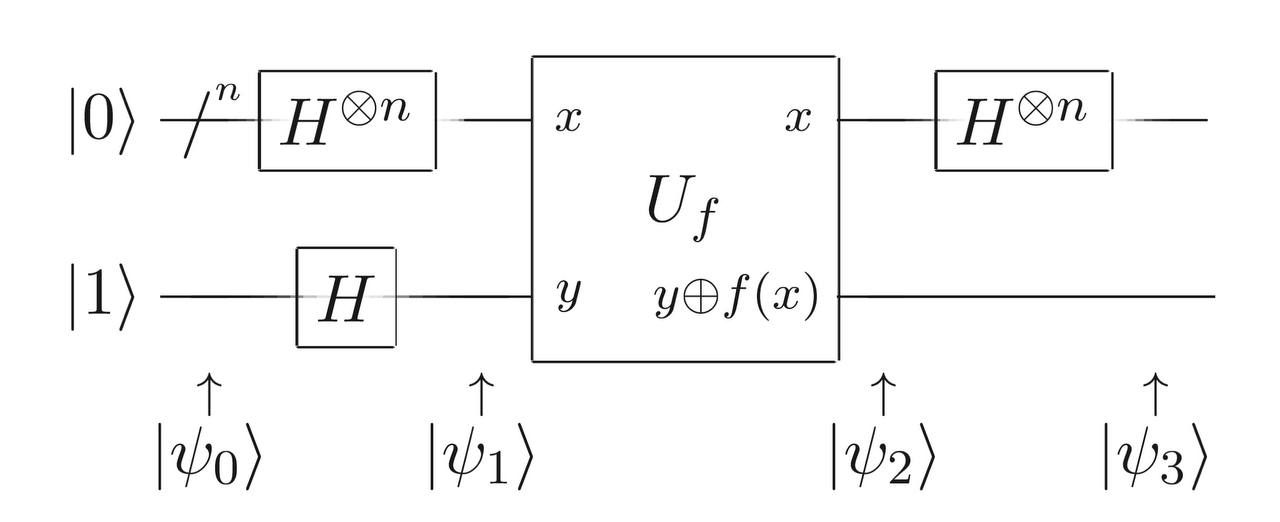
\includegraphics[width = 10cm]{./Images/dh.jpeg}
    \caption{}
    \label{fig16}
\end{figure}

La figura \ref{fig16} mostra il circuito quantistico che implementa l'algoritmo di Deutsch-Jozsa.

Analizziamo, inizialmente, il comportamento della porta di Hadamard:
\begin{equation*}
    H|a\rangle = \frac{1}{\sqrt{2}}|0\rangle + \frac{1}{\sqrt{2}}(-1)^a|1\rangle = \frac{1}{\sqrt{2}} \sum_{b \in \{0,1\}} (-1)^{ab}|b\rangle
\end{equation*}
Supponiamo ora do avere $n$ qubits eseguendo la trasformazione di Hadamard su ognuna di esse:
\begin{equation*}
\large
        \begin{array}{l}
            H^{\otimes n}|x_{n-1}\hdots x_2 x_1\rangle = \\ \\
            = \left(H|x_{n-1}\rangle\right) \otimes \hdots \otimes \left(H|x_{0}\rangle\right) = \\ \\
            = \left(\frac{1}{\sqrt{2}} \sum_{b_{n-1} \in \{0,1\}} (-1)^{x_{n-1}b_{n-1}}|b_{n-1}\rangle\right) \otimes \hdots \otimes \left(\frac{1}{\sqrt{2}} \sum_{_0 \in \{0,1\}} (-1)^{x_{0}b_0}|b_0\rangle\right) = \\ \\
            = \frac{1}{\sqrt{2^n}} \sum_{b_{n-1} \hdots b_0 \in \{0,1\}^n} (-1)^{x_{n-1}b_{n-1} + \hdots + x_{0}b_{0}} |b_{n-1}\hdots b_2 b_1\rangle
        \end{array}
\end{equation*}

Di conseguenza, abbiamo che:
\begin{equation*}
    |\psi_1\rangle = (H|1\rangle)(H^{\otimes n}|0 \hdots 0\rangle) = |-\rangle \otimes \frac{1}{\sqrt{2^n}}\sum_{b_{n-1} \hdots b_0 \in \{0,1\}^n} |b_{n-1} \hdots b_0\rangle
\end{equation*}

Eseguendo $U_f$ sullo stato, otteniamo il seguente nuovo stato:
\begin{equation*}
    |\psi_2\rangle = |-\rangle \otimes \frac{1}{\sqrt{2^n}}\sum_{b_{n-1}\hdots b_0 \in \{0,1\}^n} (-1)^{f(b_{n-1} \hdots b_0)}|b_{n-1} \hdots b_0\rangle.
\end{equation*}
Abbiamo utilizzato lo stesso fenomeno di \textit{kick-back} visto nell'algoritmo
di Deutsch.

Infine applichiamo un secondo strato di porte di Hadamard, trasformando lo stato in:
\begin{equation*}
   |\psi_3\rangle = |-\rangle \otimes \frac{1}{2^n} \sum_{b_{n-1}\hdots b_0 \in \{0,1\}^n} \sum_{c_{n-1}\hdots c_0 \in \{0,1\}^n} (-1)^{f(b_{n-1} \hdots b_0) + b_{n-1}c_{n-1} + \hdots + b_0c_0}|c_{n-1} \hdots c_0\rangle
\end{equation*}
A questo punto, dobbiamo semplicemente calcolare la probabilità che lo stato più a destra
sia esattamente uguale a $|0 \hdots 0\rangle$; infatti:
\begin{equation*}
    p(0^n) = \vert \frac{1}{2^n} \sum_{b_{n-1} \hdots b_0 \in \{0,1\}^n} (-1)^{f(b_{n-1} \hdots b_0)} \vert =
    \left\{ \begin{array}{l l}
        1 & \text{se f è }\textbf{costante} \\
        0 & \text{se f è }\textbf{bilanciata}  
    \end{array}\right.
\end{equation*}
\begin{oss}{}{}
    Osserviamo che:
    \begin{itemize}
        \item Se $f$ è \textbf{costante}, allora:
            \begin{itemize}
                \item Se $f(b_{n-1} \hdots b_0) = 0$ per una qualsiasi stringa $b_{n-1} \hdots b_0 \in \{0,1\}^n$, abbiamo che la somma è $2^n$, quindi $p(0^n) = 1$.
                \item Altrimenti, se $f(b_{n-1} \hdots b_0) = 1$, la somma è $-2^n$, quindi $p(0^n) = 1$.
            \end{itemize}
        \item Se $f$ è \textbf{bilanciata}, allora metà delle valutazioni di $f$ sono uguali ad $1$, l'altra metà sono uguali a $0$. Avremo quindi una sommatoria con numero uguali di $+1$ e $-1$, annullandosi a vicenda, facendo risultare $p(0^n) = 0$.
    \end{itemize}
\end{oss}